\documentclass{article}%
\usepackage[T1]{fontenc}%
\usepackage[utf8]{inputenc}%
\usepackage{lmodern}%
\usepackage{textcomp}%
\usepackage{lastpage}%
\usepackage[head=40pt,margin=0.5in,bottom=0.6in]{geometry}%
\usepackage{graphicx}%
%
\title{\textbf{China devela propuestas para la edición genética}}%
\author{AP}%
\date{04/03/2019}%
%
\begin{document}%
\normalsize%
\maketitle%
\textbf{URL: }%
http://www.eluniversal.com/estilo{-}de{-}vida/34338/china{-}devela{-}propuestas{-}para{-}la{-}edicion{-}genetica\newline%
%
\textbf{Periodico: }%
EU, %
ID: %
34338, %
Seccion: %
estilo{-}de{-}vida\newline%
%
\textbf{Palabras Claves: }%
NO\_TIENE\newline%
%
\textbf{Derecho: }%
2.1%
, Otros Derechos: %
\newline%
%
\textbf{\textit{La iniciativa salió luego de que un científico chino causara revuelo al anunciar que había contribuido a crear bebés con genes manufacturados}}%
\newline%
\newline%
%
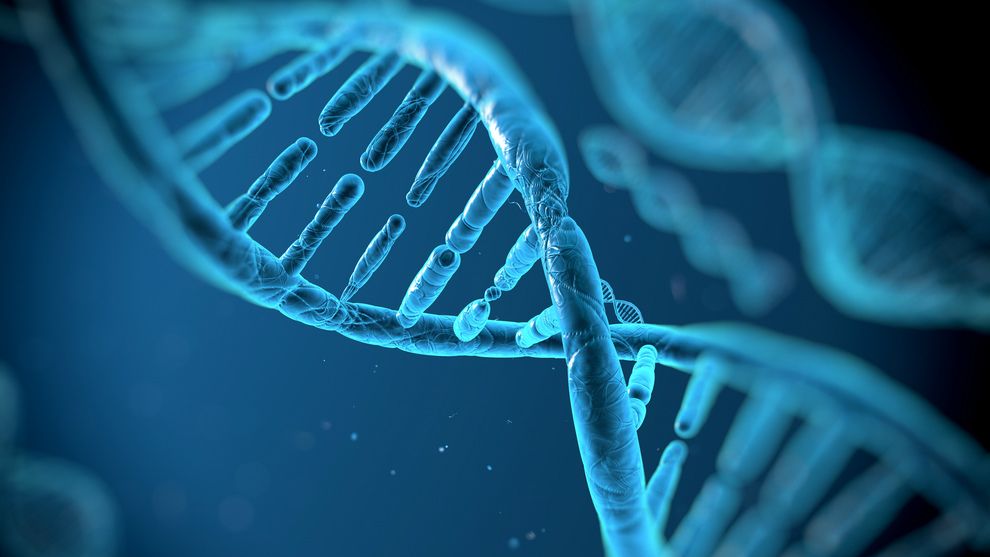
\includegraphics[width=300px]{EU_34338.jpg}%
\newline%
%
China ha develado una propuesta de nuevas normas para la edición genética y otras tecnologías biomédicas controversiales, luego que un científico chino causó revuelo al anunciar que había contribuido a crear bebés con genes manufacturados.%
\newline%
%
Bajo la propuesta entregada el martes, las tecnologías de edición genética, transferencia genética y regulación genética serán catalogadas como 'de alto riesgo' y manejadas por el departamento de salud del Consejo de Estado, el gabinete chino.%
\newline%
%
La medida surge después de que en noviembre el científico chino He Jiankui anunció que había alterado el ADN de niñas gemelas recién nacidas usando una potente nueva herramienta, según AP.%
\newline%
%
La tecnología, llamada CRISPR{-}cas9, permite manipular el ADN para suplir un gen faltante o extirpar uno que está causando problemas. \newline%
\newline%
La idea de que esa tecnología se pueda usar para crear bebés causó amplio revuelo debido a las implicaciones éticas.%
\newline%
%
Expertos denunciaron que la técnica podría haber dejado a las gemelas vulnerables a enfermedades, incluso posiblemente a infecciones virales. \newline%
\newline%
La edición genética para fines reproductivos está prohibida en Estados Unidos y en la mayor parte de Europa.%
\newline%
%
En China, las directrices oficiales prohíben toda investigación de embriones que ``viole principios éticos o morales". Las normas publicadas en el 2003 estipulan que la edición genética se permite para fines investigativos, pero que el embrión no puede pasar de los 14 días.%
\newline%
%
He Jiankui dijo en ese entonces que había editado los genes de las bebés para hacerlas inmunes al virus del sida, ya que el padre es VIH positivo. Su laboratorio estaba en Shenzhen, el centro de empresas tecnológicas en el sur de China, y reclutó a los científicos por medio de un grupo activista de defensa de pacientes de sida.%
\newline%
%
Aseguró que su objetivo era editar el ADN antes en el embrión para que los bebés sean inmunes al VIH toda su vida. \newline%
\newline%
China puso fin a los experimentos inmediatamente después de su anuncio.%
\newline%
%
Buscó también ayuda de científicos en las universidades de Stanford y Rice, donde hizo sus posgrados, y en otras instituciones, buscando asesoramiento antes y durante los experimentos.%
\newline%
%
En una entrevista con The Associated Press un mes antes de la publicación de su proyecto, el científico de 34 años de edad dijo que pensaba que la edición genética de embriones humanos incluso para nacimientos era legal en China porque no había una ley específica que lo prohibiera.%
\newline%
%
\end{document}